\subsubsection{Spectrum ROIs}

\begin{figure}[H]
    \centering
    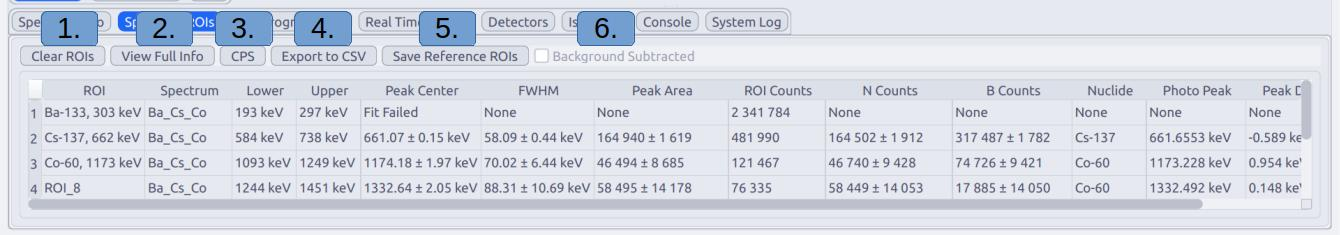
\includegraphics[width = .9\linewidth]{images/interface/spectrum_roi_info_tab.jpg}
    \caption{Spectrum ROIs tab}
    \label{fig:spectrum_rois}
    \begin{flushleft}
        \begin{enumerate}
            \item Remove all loaded ROIs from all spectra.
            \item Debug view of all data contained in the loaded ROIs.
            \item Apply time normalisation to the ROI data.
            \item Export the acquired and calculated data, including live time, of each ROI to a CSV-file.
            \item Save ROI references to the Data Library, see section \ref{sec:data_store}, for later access. These ROI references save the settings of the ROI (bounds, emission, name, fit type, etc.) but not the ROI data.
            \item Icon to display if the spectrum is background subtracted. Background subtraction effects the results of the ROI calculations.
        \end{enumerate}
    \end{flushleft}
\end{figure}